\documentclass[a4paper,12pt]{report}
\usepackage[english]{babel}
\usepackage{graphicx}
\usepackage{placeins}

\title{CLAM Documentation}
\author{Maarten van Gompel}


\newenvironment{devnotes}
{\newpage
\begin{center}
    \begin{tabular}[h!]{|p{0.8\textwidth}|}
    \hline
    {\bf Development Notes}\\\hline}
{   \\\hline
    \end{tabular}
\end{center}}


\begin{document}

\maketitle

\chapter{Introduction} 

The Computational Linguistics Application Mediator (CLAM) allows you to quickly and transparently transform your Natural Language Processing application into a webservice, with which both human end-users as well as automated clients can interact. CLAM takes a description of your system and wraps itself around the system, allowing end-users to upload input files to your application, start your application with specific parameters of their choice, and download and view the output of the application. Whilst the application runs, users can monitor its status.

CLAM is set up in a universal fashion, making it flexible enough to be wrapped around a wide range of computational linguistic applications. These applications are treated as a black box, of which only the parameters, input formats and output formats need to be described. The applications themselves need not be network aware in any way, and the handling and validation of input can be taken care of by CLAM.

CLAM is entirely written in Python and is available as open-source, it is set up in a modular fashion and as such is easily extendable. 

The kind of applications that CLAM is intended for are NLP applications, usually of a kind that do some processing on a text corpus. This corpus or smaller text can be uploaded by the user, or may be pre-installed for the webservice. The NLP application is usually expected to produce a certain output, which is subsequently made available through the webservice for viewing and downloading.

The CLAM webservice is a RESTful webservice, meaning it uses the HTTP verbs GET, POST, PUT and DELETE to manipulate resources. The principal resource in CLAM is called a project. Users can maintain various projects, each representing one specific run of the system, with specific input, output and parameters.

The webservice provides its responses in the CLAM XML format, an associated XSL stylesheet can directly transform this to xhtml in the user's browser, thus allowing both machines and people to directly communicate with the webservice.

This documentation is split into two parts: a section for service providers/developers and a section for service clients, users wanting to communicate with an existing service in an automated fashion.

\begin{devnotes}
Note that at this stage, CLAM is still under heavy development. As such, this documentation is not complete yet, but is also a work in progress.
\end{devnotes}

\chapter{Documentation for Service Providers}

\section{Technical details}

CLAM is written in Python 2.5, and is built on the webpy framework. It can run stand-alone thanks to the built-in cherrypy webserver. So no additional webserver is needed. Note that the software is designed for UNIX systems only, but any serious work in the field of NLP is UNIX based anyhow. 


\subsection{Installation}

The following software is required to run CLAM. These will be available in any modern Linux or BSD distribution:

\begin{itemize}
\item python 2.5 (or a higher 2.x version)
\item python-webpy, version 0.3
\item python-lxml, version 2 or higher
%\item python-libxslt1
%\item python-django
\end{itemize}

Each CLAM webservice will run on any TCP port of your choice. It is recommended not to use HTTP port 80. Also make sure the port is open in the firewall, at least for the machines you want to allow access.

To install CLAM, simply uncompress the clam software archive in any desired target location. The following files may be of particular interest to service providers:

\begin{itemize}
\item \texttt{clamservice.py} -- This is the webservice itself, the command to be invoked to start it.
\item \texttt{config/} -- This directory contains service configuration files. Place you service configuration here.
\item \texttt{config/defaults.py} -- This is a default configuration template which you can copy to make your own service configuration.
\item \texttt{common/} -- Common Python modules for CLAM
\item \texttt{common/parameters.py} -- Parameter-type definitions
\item \texttt{common/format.py} -- Format-type definitions
\item \texttt{static/style.css} -- The styling for visualisation

\end{itemize}

Starting the service is done by launching clamservice.py with the name of your service configuration (ucto in the example below).

\texttt{\$ ./clamservice.py clam.config.ucto}

\section{Architecture}

CLAM has a layered architecture, with at the core the NLP application(s) you want to turn into a webservice. The scheme in Figure \ref{fig:arch} illustrates the various layers: 

\begin{figure}[h]
\begin{center}
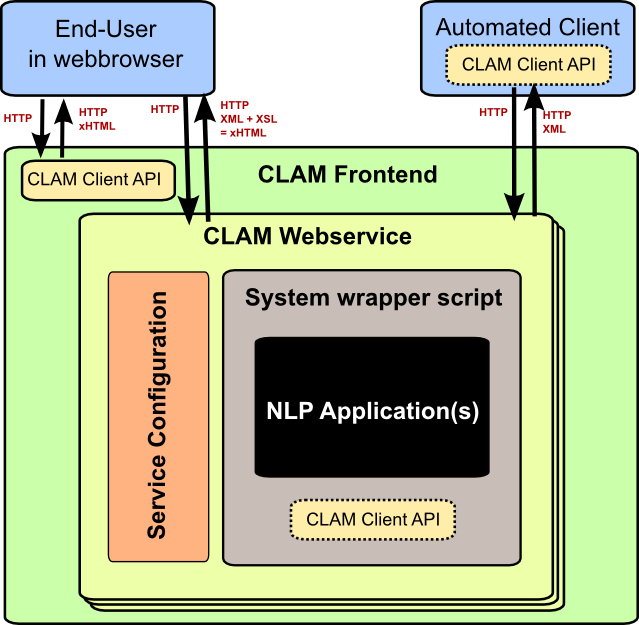
\includegraphics[width=130.0mm]{architecture.png}
\end{center}
\caption{The CLAM Architecture}
\label{fig:arch} 
\end{figure}

A CLAM webservice needs the following three components from the service developer:

\begin{enumerate}
\item A service configuration file
\item A wrapper script for your NLP application
\item An NLP application
\end{enumerate}

The wrapper script is not stricly mandatory if the NLP application can be directly invoked by CLAM. However, for more complex applications, writing a wrapper script is strongly recommended, as it offers more flexibility and better integration.

\begin{devnotes}
The CLAM Frontend, the green outer layer in Figure \ref{fig:arch} does not exist yet.
\end{devnotes}


\section{Service configuration}

The service configuration consists of a description of your NLP application, or rather, the wrapper script that surrounds it. It specifies what parameters the system can take, and what input and output formats are expected. The service configuration is itself a Python script. But due to its straightforward nature, knowledge of Python is not required to make your own.

The server configuration files reside in the \texttt{config/} directory. Making a new webservice starts with copying the sample \texttt{defaults.py} and editing your copy.

One of the first things to configure is the root path. All projects will be confined to the \texttt{projects/} directory under this root path, each project having its own subdirectory. When your NLP application or wrapper script is launched, the current working directory will be set to this project directory. Pre-installed corpora should be put in the \texttt{corpora/} directory. 
 
\subsection{Command}
\label{sec:command}

Central in the configuration file is the command that CLAM will execute. This command should start the actual NLP application, or preferably a script wrapped around it. Full shell syntax is supported and there are some special variables that will be automatically set by CLAM:

\begin{itemize}
\item \texttt{\$INPUTDIRECTORY} - The absolute path to the input directory where all the input files from the user will be stored (possibly in subdirectories). This input directory is the \texttt{input/} subdirectory in the project directory.
\item \texttt{\$OUTPUTDIRECTORY} - The absolute path to the output directory. Your system should output all of its files here, as otherwise they are not accessible through CLAM.  This output directory is the \texttt{output/} subdirectory in the project directory.
\item \texttt{\$STATUSFILE} - The absolute path to a status file. Your system may write a short message to this status file, indicating the current status. This message will be displayed to the user in CLAM's interface. The status file contains a full log of all status messages, thus your system should write to this file in append mode. Each status message consists of one line terminated by a newline character. The line may contain two tab delimited elements that will be automatically detected: a percentage indicating the progress until completion, a unix timestamp.
\item \texttt{\$PARAMETERS} - This variable will contain all parameter flags and the parameter values that have been selected by the user.
\item \texttt{\$DATAFILE} - This is the absolute path to the data file that CLAM outputs in the project directory. This data file, in CLAM XML format, contains all parameters along with their selected values. Furthermore it contains the inputformats and outputformats, and a listing of uploaded input files and/or pre-installed corpora. System wrapper scripts can read this file to obtain all necessary information. If the system wrapper script is written in Python, the CLAM Client API can be used to read this file, requiring little effort on the part of the developer.
\item \texttt{\$USERNAME} - The username of the logged in user.
\end{itemize}


Make sure the actual command is an absolute path or the executable is in the user's \texttt{\$PATH}. Upon launch, the current working directory will be automatically set to the specific project directory. Within this directory, there will be an \texttt{input/} and \texttt{output/} directory, but use the full path as stored in \texttt{\$INPUTDIRECTORY} and \texttt{\$OUTPUTDIRECTORY}/. All uploaded user input will be in this input directory, and all output that users should be able to view or download, should be in this output directory.

\subsection{Parameters}
\label{sec:parameters}

The parameters which an NLP application, or rather the wrapper script, can take, are defined in the service configuration. First of all parameters can be subdivided into parameter groups, but these serve only presentational purposes. 

Parameters of six types are predefined, though other types can be added to \texttt{common/parameters.py}. Each is a Python class taking the following mandatory arguments:

\begin{enumerate}
\item \textbf{\texttt{id}} -- An id for internal use only.
\item \textbf{\texttt{paramflag}} -- The parameter flag, this flag will be added to \texttt{\$PARAMETERS} when the parameter is set. It is customary for parameter flags to consist of a hyphen and a letter or two hyphens and a string. Parameter flags could be for example be formed like: \texttt{-p} ,\texttt{--pages}, \texttt{--pages=}. There will be a space between the parameter flag and its value, unless it ends in a \texttt{=} sign or \texttt{nospace=True} is set. Multi-word string values will automatically be enclosed in quotation marks, for the shell to correctly parse them. Technically, you are also allowed to specify an empty parameter flag, in which case only the value will be outputted, as if it were an argument.
\item \textbf{\texttt{name}} -- The name of this parameter, this will be shown to the user in the interface.
\item \textbf{\texttt{description}} -- A description of this parameter, meant for the end-user.
\end{enumerate}


The six parameter types are:

\begin{itemize}
\item \textbf{\texttt{BooleanParameter}} - A parameter that can only be turned on or off, represented in the interface by a checkbox. If it is turned on, the parameter flag is included in \texttt{\$PARAMETERS}, if it is turned off, it is not. If \texttt{reverse=True} is set, it will do the inverse.
\item \textbf{\texttt{IntegerParameter}} - A parameter expecting an integer number. Use \texttt{minrange=}, and \texttt{maxrange=} to restrict the range.
\item \textbf{\texttt{FloatParameter}} - A parameter expecting a float number. Use \texttt{minrange=}, and \texttt{maxrange=} to restrict the range.
\item \textbf{\texttt{StringParameter}} - A parameter taking a string value. Use \texttt{maxlength=} if you want to restrict the maximum length.
\item \textbf{\texttt{TextParameter}} - A parameter taking multiple lines of text. 
\item \textbf{\texttt{ChoiceParameter}} - A multiple-choice parameter. The choices must be specified as a list of \texttt{(ID, label)} tuples, in which ID is the internal value, and label the text the user sees. For example, suppose a parameter with flag \texttt{-c} is defined.  \texttt{choices=[('r','red'),('g','green'),('b', 'blue)]}, and the user selects ``green'', then  \texttt{-c g} will be added to \texttt{\$PARAMETERS}. The default choice can be set with \texttt{default=}, and then the ID of the choice. If you want the user to be able to select multiple parameters, then you can set the option \texttt{multi=True}. The IDs will be concatenated together in the parameter value, a delimiter (a comma by default) can be specified with \texttt{delimiter=}. If you do not use \texttt{multi=True}, but you do want all options to be visible in one view, then you can set the option \texttt{showall=True}.
\end{itemize}

All parameters can take the following extra named arguments:

\begin{itemize}
\item \textbf{\texttt{default}} - Set a default value.
\item \textbf{\texttt{required}} - Set to \texttt{True} to make this parameter required rather than optional.
\item \textbf{\texttt{require}} - Set this to a list of parameter IDs. If this parameter is set, so must all others in this list.
\item \textbf{\texttt{forbid}} - Set this to a list of parameter IDs. If this parameter is set, none of the others in the list may be set.
\item \textbf{\texttt{allowusers}} - Allow only the specified lists of usernames to see and set this parameter. If unset, all users will have access. You can decide whether to use this option or \texttt{denyusers}, or to allow access for all.
\item \textbf{\texttt{denyusers}} - Disallow the specified lists of usernames to see and set this parameter. If unset, no users are blocked from having access. You can decide whether to use this option or \texttt{allowusers}, or to allow access for all.
\end{itemize}
%TODO


\subsection{Inputformats \& Outputformats}
\label{sec:formats}

CLAM takes care of the handling of input and output formats. When a user uploads a file, he chooses from a list of options to select the desired input format. Each inputformat is associated with a particular extension. CLAM automatically renames the uploaded files so they get the desired extension, relieving the end-user of this burden. If multiple extensions are defined the first is used. An extension is also associated with each outputformat, the system output files are recognised on the basis of this extension. Your system wrapper can recognise file formats also on the basis of their extension, or by explicitly getting their format from the \texttt{clam.xml} datafile. Moreover, input formats and output formats can also have associated validators, which can check if the file really is in the desired format. And for each inputformat and outputformat, a character encoding needs to be explicitly set.

The inputformats are defined in the service configuration file as a list of classes, where each class corresponds to a particular input format. The outputformats are defined in a similar way. The classes themselves are defined in \texttt{common/formats.py}, where you can add any new types (subclassed from \texttt{Format}).

Defining a format goes as follows, let's take PlainTextFormat as example:

\begin{verbatim}
INPUTFORMATS = [ PlainTextFormat('utf-8' ['.txt'], subdirectory='texts' ) ]
\end{verbatim}

The first argument of the class constructor is the encoding, the second is a list of acceptable extensions, of which the first will be used in the rename procedure. You can redeclare instances of the same format with different encodings, but make sure the extensions you specify are unique. Some extra arguments can be provided:

\begin{itemize}
\item \textbf{\texttt{subdirectory=}} -- Store all files of this format in the specific subdirectory of the input directory. This allows you to separate files of a certain format into distinct directories. 
\item \textbf{\texttt{archivesubdirs=}} -- Set this to False if you want to extract archives in a flattened fashion, with disregard for any subdirectories therein.
\end{itemize}

Note that users can upload either single files in the specified format, or an archive (\texttt{zip}, \texttt{tar.gz} or \texttt{tar.bz2}) containing multiple files in the specified format. 

\subsection{Users}

Being a RESTful webservice, user authentication proceeds over HTTP itself. CLAM implements HTTP Digest Authentication, which as opposed to Basic Authentication computes a hash of the username and password client-side and transmits that hash, rather than a plaintext password. 

A list of users can be defined in \texttt{USERS} in the service configuration file, this is a dictionary of usernames mapped to an md5 hash computed on the basis of the username, the system ID, and the password. Furthermore there is a setting \texttt{PROJECTS\_PUBLIC}, which can be set to \texttt{True} or \texttt{False}, in the former case all projects will be open to all authenticated users, in the latter case projects will only be accessible by their owners.

User authentication is not mandatory. But for any world-accessible environment it is most strongly recommended, for obvious security reasons.

The ability to view and set parameteres can be restricted to certain users, you can use the extra parameter options \texttt{allowusers=} or \texttt{denyusers=} to set this. See section \ref{sec:parameters}. A common use would be to define one user to be the guest user, for instance the user named ``guest'', and set \texttt{denyusers=['guest']} on the parameters you don't want the guest user to use.

\begin{devnotes}
Eventually, an option will probably be implemented to read users from a database. HTTPS support may also be added at a later stage.
\end{devnotes}

\section{Wrapper script}

Service providers are encouraged to write a wrapper script that acts as the glue between CLAM and the NLP Application(s). CLAM will execute the wrapper script and the wrapper script will invoke the actual NLP Application(s). Using a wrapper script offers more flexibility than letting CLAM directly invoke the NLP Application, and allows the NLP Application itself to be totally independent of CLAM. 

The wrapper script takes the arguments as selected for \texttt{COMMAND} in the service configuration file. There are some important things to take into account:

\begin{itemize}
\item All user-controllable input has to be read from the specified input directory. If you do not use the \texttt{clam.xml} data file, then you have to determine the file's format based on its extension. See Section \ref{sec:formats}.
\item All user-viewable output must be put in the specified output directory. Make sure your system outputs files with an extension CLAM will recognise. See \texttt{\$OUTPUTFORMATS} in Section \ref{sec:formats}.
\item The wrapper should periodically output a small status message to \texttt{\$STATUSFILE}. 
\item The wrapper script is always started with the current working directory set to the selected project directory.
\end{itemize}

The wrapper script can be written in any language. Python developers will have the big advantage that they can directly tie into the CLAM Client API, which handles things such as reading the \texttt{clam.xml} data file.

\begin{devnotes}
CLAM Client API will be further discussed, possibly in next chapter.
\end{devnotes}

\chapter{Documentation for Service Clients}

\begin{devnotes}
Yet to be written... %TODO
\end{devnotes}


%\section{Resource oriented approach}

%Being a RESTful webservice, CLAM has a resource-oriented approach. 


\end{document}
